\section{Framework}
This section will describe all of the parts that make the framework. Figure~\ref{fig:framework}.

\begin{figure}[tb] 
\centering
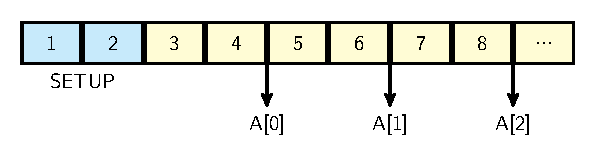
\includegraphics[width=\columnwidth]{images/l2_model.pdf}
\caption{\small Example of Layer 2 memory burst access.}
\label{fig:framework}
\end{figure}

\subsection{Application}
The framework can take as input a streaming application. The framework performs an exact data dependency analysis on the application, hence the behaviour of the application needs to be completely specified at compile time. Listing~\ref{lst:matrixvec} shows the application source code that will be used for the remainder of this paper. The language that the framework currently supports is C/C++, however the framework uses the LLVM Intermediate Representation CITATION NEEDED, so the support for other languages can be easily added.
\begin{lstlisting}[language=C, caption={Example of input application, C implementation of a matrix vector multiplication.}, label={lst:matrixvec}]
void matrix_vec_kernel(int *A,int *B, int *C){
    int sum;
    for(int i=0;i<DIM2;i++){
        sum=0;
        for(int j=0;j<DIM1;j++){
            sum+=A[i*DIM1+j]*B[j];
        }
        C[i]=sum;
    }
}
\end{lstlisting}

\subsection{Configuration File}
The second input to the framework is a configuration file. The Configuration file contains a description of the different component to be used in the realization of the hardware architecture, an example is shown in Listing~\ref{conf_file}. Using this file the user can specify the process technology to be used - e.g. 16nm, 28nm - the clock frequency of Layer 1 memory, Layer 2 memory and Custom Processor. The user can moreover specify the datawidth used by the different operators - e.g. multipliers, adders-, and by the Layer 1 and Layer 2 memory. 
Detailed information requred to model the Layer 2 burst accesses are as well contained in this file: the setup latency for write/read accesses, the type of Layer 2 memory to be used -e.g. MRAM, SRAM etc..- and the size of the Layer 2 memory.
\begin{lstlisting}[language=json, caption={Example of input configuration file}, label={lst:conf_file}]
{ 
   "resource_database": { 
	"technology": 16, 
	"clock_frequency": 1000, 
	"bitwidth_adder": 128, 
	"bitwidth_multiplier": 64, 
	"bitwidth_register_file": 128, 
	"type_l2": "tt1v1v85c", 
	"technology_l2": 16, 
	"clock_l2": 800, 
	"bitwidth_l2": 32, 
	"depth_l2":2048, 
	"setup_write_latency_l2":2, 
	"setup_read_latency_l2":2 
   } 
}

\end{lstlisting}

\subsection{Layer 2 Read Model}
\subsection{Data Dependency Analysis}
\subsection{Maximal Parallel Architecture and Maximal Sequential Architecture}
\subsection{Design Space Exploration}
\subsection{Layer 2 Write Model}
\subsection{Architecture Tradeoffs}

